\documentclass[]{article}
\usepackage[utf8]{inputenc}
\usepackage{amsthm}
\usepackage{amssymb}
\usepackage{amsmath}
\usepackage{calc}
\usepackage{tikz}
\begin{document}
\begin{center}
\begin{tikzpicture}
\def\f{0.015}
\def\ra{\f*300}
\def\ri{\f*75}
\def\rm{\f*160}
\def\d{\f*20}
\draw (0,0) circle (\ra) node {};
\draw (0,0) circle (\ri) node {};
\draw (0,\rm) circle (\d) node {};
\draw (0,-\rm) circle (\d) node {};
\draw (\rm,0) circle (\d) node {};
\draw (-\rm,0) circle (\d) node {};
\end{tikzpicture}
\end{center}
\begin{align*}
u_r&=C_1r+\frac{C_2}{r}-\frac{1-v^2}{8E}\varrho\omega^2r^3+(1+v)\frac{\alpha}{r}\int_{a}^{r}r'\Delta Tdr'\\
\sigma_r&=\frac{E}{1-v}C_1-\frac{E}{(1+v)r^2}C_2-\frac{3+v}{8}\varrho\omega^2r^2+\frac{E\alpha}{r^2}\int_{a}^{r}r'\Delta Tdr'\\
\sigma_\varphi&=\frac{E}{1-v}C_1+\frac{E}{(1+v)r^2}C_2-\frac{1+3v}{8}\varrho\omega^2r^2+E\alpha(\Delta T-\frac{1}{r^2}\int_{a}^{r}r'\Delta Tdr')
\end{align*}
Aus $\omega=0$ und $\Delta T=0$ folgt:
\begin{align*}
u_r&=C_1r+\frac{C_2}{r}\\
\sigma_r&=\frac{E}{1-v}C_1-\frac{E}{(1+v)r^2}C_2\\
\sigma_\varphi&=\frac{E}{1-v}C_1+\frac{E}{(1+v)r^2}C_2
\end{align*}
Gegeben sind $\sigma_r(r_1)=\sigma_1$ und $\sigma_r(r_2)=\sigma_2$. Damit kann man $C_1$ und $C_2$  herleiten:
\begin{align*}
C_1&=(1-v)\left( \frac{\sigma_2}{E}+\frac{C_2}{(1+v)r_2^2}\right) \\
C_2&=\frac{(\sigma_1-\sigma_2)r_1^2r_2^2(1+v)}{E(r_1^2-r_2^2)}
\end{align*}
Mit $\sigma_1=-100N/mm^2$ und $\sigma_2=0N/mm^2$ folgt:
\begin{align*}
C_1&\approx-3,73\cdot 10^{-4}\\
C_2&=-3,9mm^2
\end{align*}
\def\CA{-0.000373} %0.0000233
\def\CB{-3.9} %3.9
\def\E{4000}
\def\sigR{(\CA/0.7-\CB/(1.3*((x*25)+75)*((x*25)+75)))}
\def\sigP{(\CA/0.7+\CB/(1.3*((x*25)+75)*((x*25)+75)))}
\def\sigT{-106.7/200000}
Tangetial- und Radialspannung\\
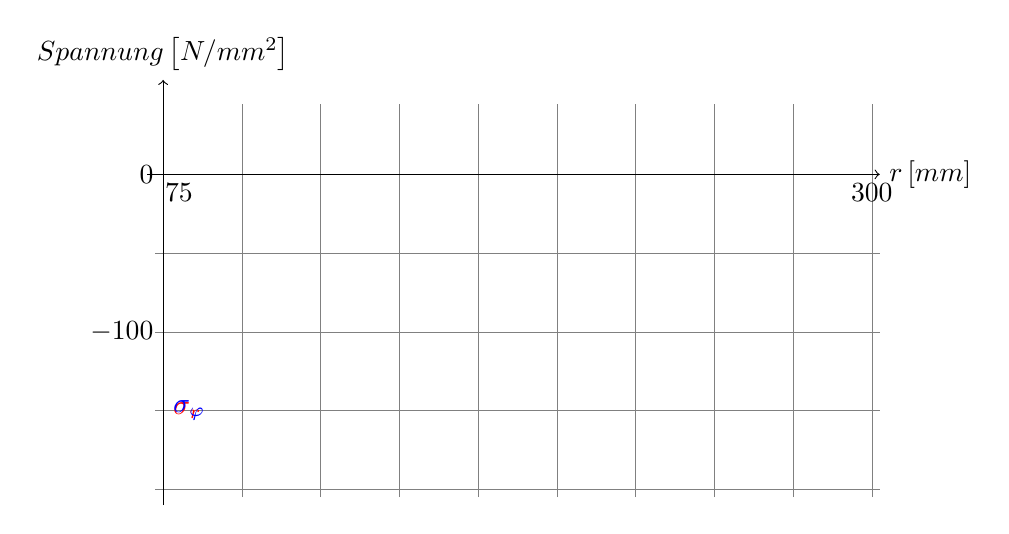
\begin{tikzpicture}[domain=0:9]
    \draw[very thin,color=gray] (-0.1,-1.1) grid (9.1,3.9);
    \draw[->] (-0.2,3) -- (9.1,3) node[right] {$r\left[ mm\right] $};
    \draw[->] (0,-1.2) -- (0,4.2) node[above] {$Spannung \left[ N/mm^2\right]$};
    \draw[color=red,thick] plot[id=x] function{\E*\sigR+3} 
            node[right] {$\sigma_r$};
    \draw[color=blue,thick] plot[id=x] function{\E*\sigP+3} 
                        node[right] {$\sigma_\varphi$};
    \draw (0,1) node[left] {$-100$};
    \draw (0,3) node[left] {$0$};
    \draw (0.2,3) node[below] {$75$};
    \draw (9,3) node[below] {$300$};
\end{tikzpicture}\vspace{1cm}\\
Vergleichsspannung
$$\sigma_v=\sqrt{\sigma_r^2+\sigma_\varphi^2+\sigma_t^2-\sigma_r\sigma_\varphi-\sigma_t\sigma_\varphi-\sigma_r\sigma_t}$$
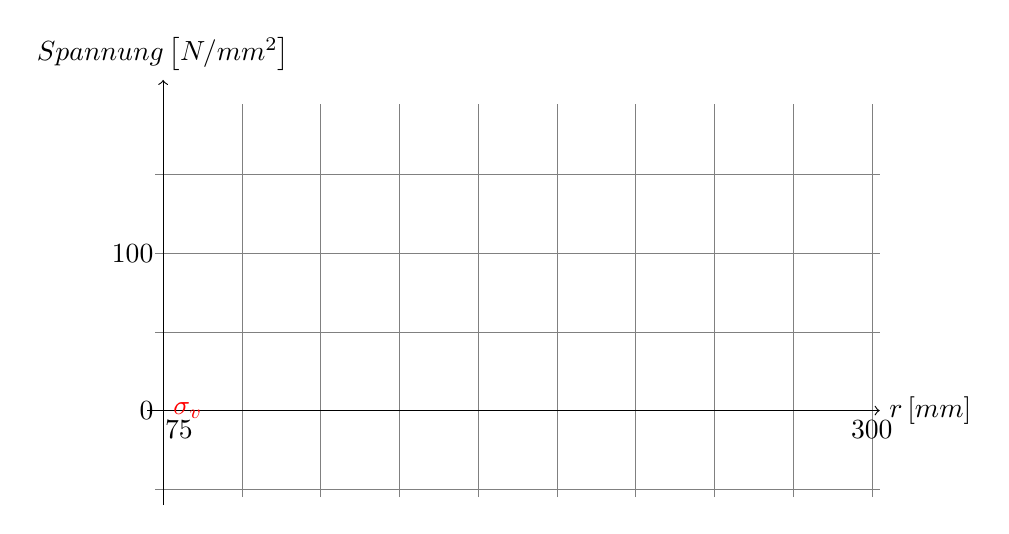
\begin{tikzpicture}[domain=0:9]
    \draw[very thin,color=gray] (-0.1,-1.1) grid (9.1,3.9);
    \draw[->] (-0.2,0) -- (9.1,0) node[right] {$r\left[ mm\right] $};
    \draw[->] (0,-1.2) -- (0,4.2) node[above] {$Spannung \left[ N/mm^2\right]$};
    \draw[color=red,thick] plot[id=x] function{4000*sqrt(\sigR*\sigR+\sigP*\sigP+\sigT*\sigT-\sigP*\sigR-\sigT*\sigR-\sigP*\sigT)} 
                            node[right] {$\sigma_v$};
    \draw (0,0) node[left] {$0$};
    \draw (0,2) node[left] {$100$};
    \draw (0.2,0) node[below] {$75$};
    \draw (9,0) node[below] {$300$};
\end{tikzpicture}\\
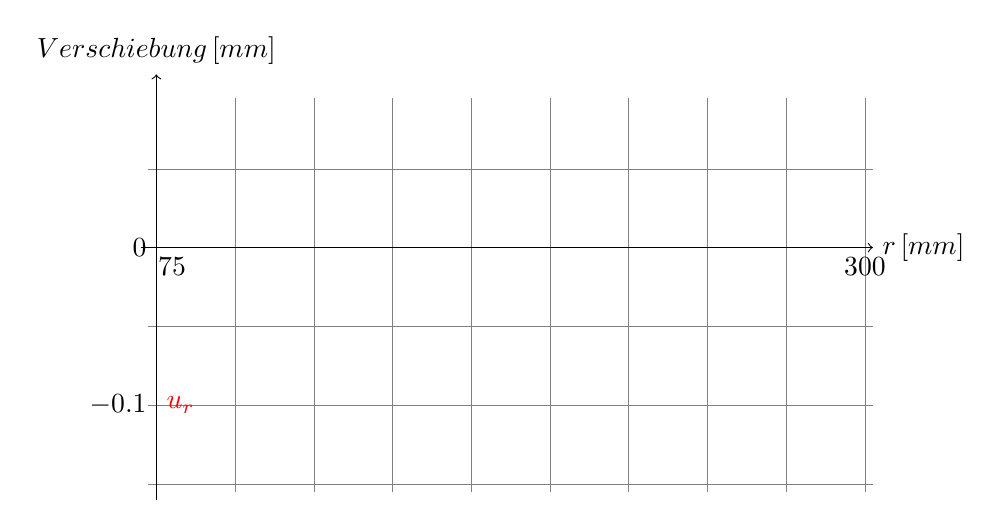
\begin{tikzpicture}[domain=0:9]
    \draw[very thin,color=gray] (-0.1,-1.1) grid (9.1,3.9);
    \draw[->] (-0.2,2) -- (9.1,2) node[right] {$r\left[ mm\right] $};
    \draw[->] (0,-1.2) -- (0,4.2) node[above] {$Verschiebung \left[ mm\right]$};
    \draw[color=red,thick] plot[id=x] function{20*(\CA*((x*25)+75)+\CB/((x*25)+75))+2} 
        node[right] {$u_r$};
    \draw (0,0) node[left] {$-0.1$};
    \draw (0,2) node[left] {$0$};
    \draw (0.2,2) node[below] {$75$};
    \draw (9,2) node[below] {$300$};
\end{tikzpicture}
\end{document}
